\chapter{Das Problem}
Das Open Pouring Problem wird formal wie folgt beschrieben: Es seien drei Krüge mit unterschiedlichen Kapazitäten gegeben, die jeweils eine ganzzahlige Menge an Wasser enthalten. 
In jedem Schritt darf eine Wassermenge, die höchstens der aktuellen Wassermenge eines Kruges entspricht, von einem Krug in einen anderen gegossen werden. Das Ziel ist es, durch eine Reihe solcher Schritte einen der Krüge vollständig zu leeren, das heißt, seine Wassermenge auf null zu reduzieren.

\begin{figure}[H]
    \centering
    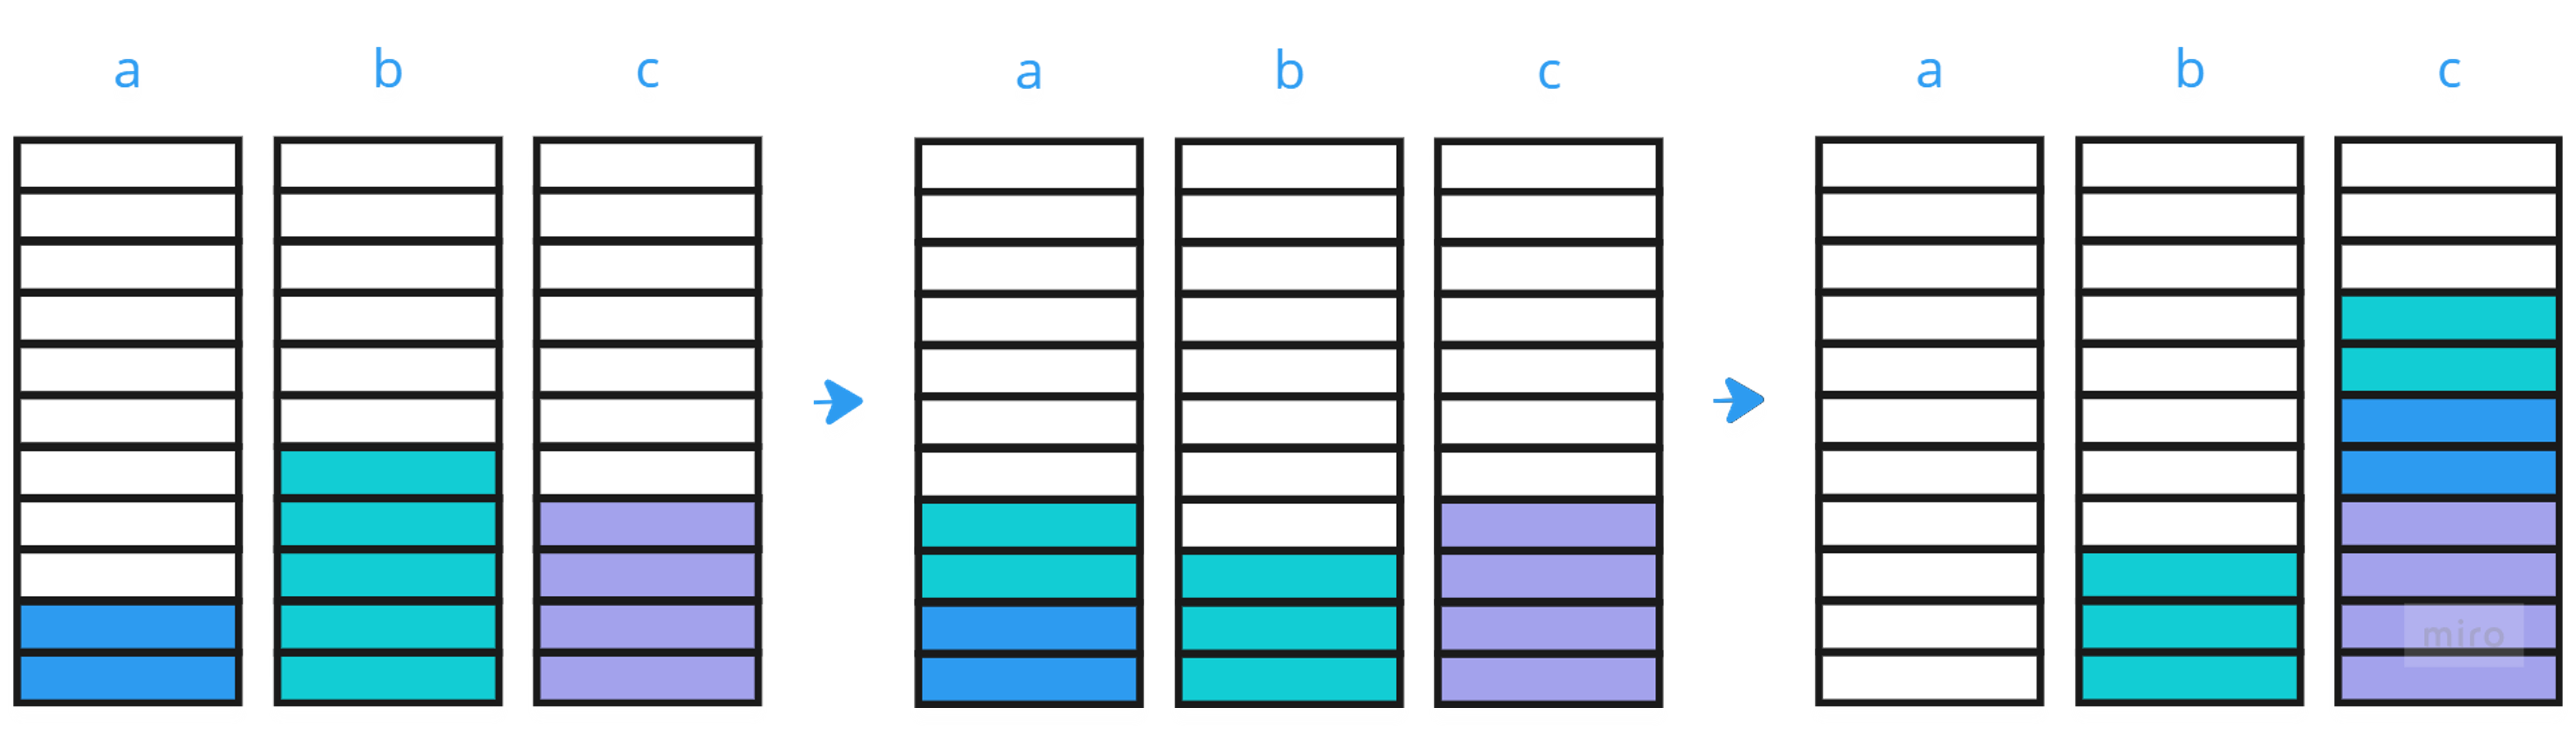
\includegraphics[page=1, width=1\textwidth]{./bilder/Pouring_Problem_1.png} 
    \caption{Pouring Problem: ein einfaches Beispiel mit zwei, fünf und 4 Litern in der Anfangskonfiguration} 
    \label{fig:pouring_problem_die_hard}
\end{figure}

Die mathematische Modellierung des Problems erfolgt durch die Definition einer Konfiguration als Tripel $(a, b, c)$, wobei $a$, $b$ und $c$ die Wassermengen in den drei Krügen darstellen. Das Problem besteht darin, eine Sequenz von Operationen zu finden, die eine Ausgangskonfiguration $(a, b, c)$ in eine Endkonfiguration $(a', b', 0)$ überführt. Die Herausforderung liegt darin, die minimale Anzahl der erforderlichen Schritte zu bestimmen, die in allen möglichen Konfigurationen benötigt werden. \\

\autocite{Frei.2020} % ToDo wo überall die Quelle hinzufügen, oder das irgendwo ganz am Anfang einfach rein schreiben?